\documentclass[12pt]{template}
\usepackage{fancyhdr}
\begin{document}
\section{使用事件描述预测事件参与人数}
\subsection{概述}
上一章证明了事件描述对事件参与人数有显著的影响,因此,通过事件描述来预测参与人数便是顺理成章的了。 所以,接下来本章会提出三种预测器来预测二者之间的关系。这三种预测器分别是线性回归,带卷积层的神经网络和带GRU的神经网络。接下来,本章将分别对这三个预测器进行详细的描述。

\subsection{线性回归预测器}
线性回归是最简单的一种回归方法,同时只要二者关系是正相关的,在大多数情况下线性回归也有着不错的效果,所以这里也是把线性回归作为选择之一的原因。同时,线性回归也是本次实验的基线。在实验中,我们并没有采用最传统的线性回归,而是采用了拉索回归。原因是上一章我们假设事件描述对事件参与人数的影响主要由描述中的某些词导致的。所以这里在损失函数中加入L1正则来突出某些词的作用。此预测器及其损失函数如下:
% lasso function
\begin{equation}
argmin\left\{\frac{1}{N}\displaystyle\sum_{i=1}^{N}
(y_i-\beta_0-\displaystyle\sum_{j}\beta_jx_{ij})^2\right\}
\end{equation}
\begin{equation}
subject\ to \quad \displaystyle\sum_{i}|\beta_i|<\alpha
\end{equation}
\begin{equation}
loss\ function: MSE+\sigma*\sum|\beta|
\end{equation}

在实现中,为了与后面两个分类器统一,我们使用了输出维数为1的单层线性神经网络,并采用了\textit{l1}正则。预测器的输入是序列化后的文本,目标(\textit{target})及输出则是参与人数。

\subsection{带卷积层的神经网络}
在使用线性回归做预测器时,我们假设各属性对结果的影响是互相独立,不受出现顺序影响的,即\(d(w|s_0)=d(w|s_0')=d(w)\),其中\textit{w}为词,\(s_0,s_0'\)为不同排列的相同的文本序列,\textit{d}为某个不存在的影响函数。但显然这个假设在现实中是不成立的,在自然语言中,词的出现顺序是非常重要的信息。例如在一段事件描述中,\textit{we will hold the meeting in a church}与\textit{church a in meeting the hold will we}这两句话在线性规划的眼中是没有区别的,但显然以人的眼光看,第二句话是没有意义的。因此,为了将文本的序列信息纳入考量范围,这里我们参考了seqGan\ref{yu_seqgan:_2016}中判别器的结构,设计了如下了带卷积的神经网络,如图\ref{f21}

我们首先将输入文本\(w_0,w_1,...,w_t\)表示成如下形式:
\begin{equation}
S_{0:t}=x_0\oplus x_1\oplus...\oplus x_t
\end{equation}

其中,\(x_i\)为\(w_i\)对应的\textit{k}维词向量\(\subseteq R^k\),\(\oplus\)是拼接符号,\(S_{0:t}\)是一个\(t\times k\)的矩阵。然后我们使用若干个卷积核\(k\subseteq R^{l\times k}\)对窗口大小为\textit{l}中的词进行卷积操作,产生一个新的特征向量。
\begin{equation}
c_i=\rho(w\otimes S_{i:i+l-1}+b)
\end{equation}
\(\otimes\)为元素乘积之和,\textit{b}为偏移量,\(\rho\)为非线性函数。在实现中我们可以使用多个相同尺寸的核来进行卷积,然后对得到的不同的\(c_i\),即\textit{max-pooling}。(例如图\ref{f21}中第一个卷积核的\textit{l}为3,使用了4个不同的卷积核,即对于相同的窗口一次输出四个结果,然后在这四个结果中取最大值,即为窗口大小为\textit{l}所对应的最终卷积结果。)为了得到不同窗口尺寸下的上下文关系,我们也可以使用不同尺寸的核。最后,我们将结果拼接起来,得到处理后的特征向量。送入下一个环节。下一个环节为带隐含层的线性网络,假设得到最终的特征向量为\(\hbar\subseteq R^{k'}\)(图中对应的\textit{k}为9),那么接下来我们对\(\hbar\)进行如下操作。
\begin{equation}
\hbar'=\sigma(w_0\cdot\hbar+b_0)
\end{equation}
\begin{equation}
output = w_1\cdot\hbar'+b_1
\end{equation}

\(w_0,w_1\)分别对应第一和第二个蓝色方块,\(\sigma\)为非线性函数,\(\cdot\)为矩阵乘法运算。

关于该网络的损失函数,为了最小化预测结果和目标的误差,我们使用了均方误差损失函数,并对最后两个线性神经网络采用了\textit{l2}正则\ref{eq1}。这里采用\textit{l2}正则的原因是我们希望最后的线性神经网络能尽可能的考虑前面卷积神经网络输出的所有维度,而不是过度的依赖某些维度。
\begin{equation}\label{eq1}
loss=\frac{1}{N}\displaystyle\sum_{i=1}^{N}\left\{(y_i-y'_i)^2\right\}+\alpha||w_0^2||+\beta||w_1^2||
\end{equation}
\begin{figure}[htbp]
    \centering
    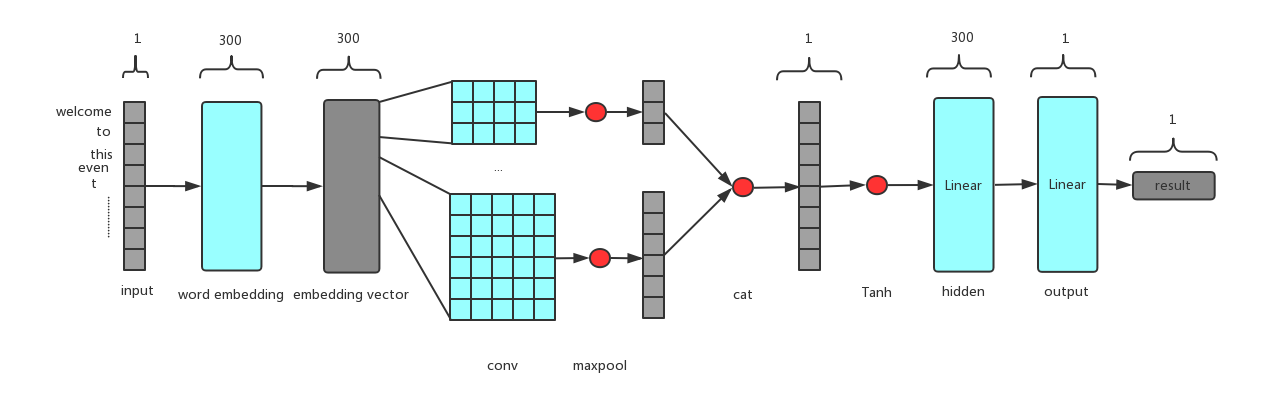
\includegraphics[width=16cm]{conv_ranker.png}
    \caption{带卷积层的神经网络}
    \captionsetup{font=small,margin=30pt}\caption*{图中灰色的方块表示向量,蓝色的表示网络,红色的圆点表示算符。在计算过程中,输入是文本序列,然后首先经过词向量层转换成词向量,然后进行卷积和池化(\textit{max-pooling}),将结果拼接起来,然后使用双曲正切(\textit{tanh})归一话,最后经过一个带隐含层的线性前馈神经网络输出最终结果。}
    \label{f21}
\end{figure}

\subsection{带GRU的神经网络}
在上一小节,我们使用了卷积层对原始输入文本转换成的词向量进行了处理,得到了一个新的特征向量。这个过程也可以看成是定义了一个函数\(f:R^{m\times k}\mapsto R^n\),将原本在\(R^{m\times k}\)空间中的样本映射/编码到了\(R^n\)中。这样做的目的是可以方便后续处理,这里我们相当于把一条文本转换成了一个向量,接下来的工作就在这向量上展开了。但如何去找到一个这样的函数\textit{f},则是这种方法成败的关键。在这篇论文中,我们希望\textit{f}有如下的特点:1)能处理序列信息。2)能在转换过程中尽量保留原始信息。3)方便,易于实现。而我们之前使用的卷积层并不完全满足这三个条件。首先,它能处理序列信息,但只能考量到同在一个窗口大小内的序列,而且就算在同一个窗口内,它也不会考虑其出现顺序。换而言之,它能处理序列信息是基于这些词出现在不同的窗口来保证的,如果不能合适的设置窗口大小,就不能捕获我们想要的序列信息。而在文本处理中,如何设置窗口大小是件困难的事情。其次,因为池化层的存在,它在转换过程中能保留多少原始信息是存疑的。最后,它实现起来挺容易,这点没有问题。

而另一种处理时序信息的网络结构循环神经网络,则可以很好的满足上面三个条件。
\end{document} 